
%(BEGIN_QUESTION)
% Copyright 2013, Tony R. Kuphaldt, released under the Creative Commons Attribution License (v 1.0)
% This means you may do almost anything with this work of mine, so long as you give me proper credit

Calculate the temperature of the process if the voltmeter registers 12.991 mV when connected to the transmitter terminals:

$$\includegraphics[width=15.5cm]{i02897x01.eps}$$

$T_{process}$ = \underbar{\hskip 50pt} degrees F

\underbar{file i02897}
%(END_QUESTION)





%(BEGIN_ANSWER)

$T_{process}$ = \underbar{\bf 649} degrees F
 
%(END_ANSWER)





%(BEGIN_NOTES)

{\bf This question is intended for exams only and not worksheets!}.

%(END_NOTES)


